\scanpage{81}

\(I'_{f'}\quad (f_{i'}:\mathcal E_{i'}\longrightarrow
\mathcal E_{i=\tau(i')},\ \text{les }\alpha_{i'}\in\mathcal E)\)
sont pareils que dans le cas envisagé précédemment.

\uline{NB} Cela signifie en fait qu'on commence \unsure{à} "boucher les trous" \deleted{de}
(de \(X'\)) correspondants aux \(i'\in I'\setminus I'_{f'}\), en remplaçant
\(\mathcal E'\) par le \deleted{\unsure{ss-}}groupe quotient de \(\mathcal E'\)
par le ss-groupe invariant engendré par les
\(L_{i'}=\kappa_{i'}(T(\overline K))\)
\((i'\in I'\setminus I'_{f'})\), et \deleted{les} \unsure{\(\mathcal E_{i'}\)}
\((i'\in I'_{f'})\) par leurs images dans ledit groupe quotient, et en oubliant
\deleted{les} \(I'\setminus I'_{f'}\), i.e. remplaçant \(I'\) par \(I'_{f'}\).

[Pour bien faire, il faudrait exprimer ces opérations aussi au niveau des diagrammes
de groupoïdes
\diagram{\begin{tikzcd}[ampersand replacement=\&]
\Pi'_{\unsure{D^*}} \arrow[r,dash] \& \Pi'_U \arrow[r] \& \unsure{\Pi'_e|\Pi_e}
\end{tikzcd}}
\(\ldots\)].

\margin{\deleted{\illegible{2} il faudrait encore \unsure{expliciter}
\illegible{2} \unsure{des|les} pts de \illegible{1}}}

Cela signifie donc qu'en fait, on s'est ramené à la situation envisagée au début,
où \(S'=\widehat f^{-1}(S)\)\ldots\ Donc finalement
la différence des deux pts de vue n'est pas énorme, et
\deleted{\illegible{1}}\inserted{celui} adopté au début a l'avantage de
la simplicité plus grande (tout est relatif !)

\margin{80}

\scanpage{82}
\mspage{39}

11. Conditions sur les systèmes de \deleted{\unsure{diagrammes}}\inserted{groupoïdes}
obtenus à partir de situations géométriques.

On en a déjà cité au passage, p.ex. que les groupes noyaux de
\(\Pi_{D^*}-\Pi_e\) sont abéliens (avec l'isom de Kummer \(\kappa\))
et que les images sont des sous-groupes ouverts, et de \(=\) pour
l'image des \deleted{\illegible{1}} \(\pi_1\) dans \(\Pi_U-\Pi_e\).
On va réexpliciter \inserted{et préciser} ceci dans le cadre de l'interprétation
en termes de
\diagram{\begin{tikzcd}[ampersand replacement=\&]
T(\overline K) \arrow[r,"\kappa_i"] \& \mathcal E_i \arrow[r,hook,"\rho_i"] \&
\mathcal E \arrow[r,"p"] \& \Gamma
\end{tikzcd}}
(cas de la "dim 1" --- on n'exclut pas le cas \(I=\varnothing\) ---
le cas "dim 0" étant trivial\ldots)

a) L'image \inserted{\(\Sigma\)} de \(p\) est ouverte, plus précisément existe
ss-groupe ouvert \(\Gamma'\subset\Gamma\) au dessus duquel
\(\mathcal E\) ait une section [et = une "section admissible" en un sens qui sera
défini par la suite --- de sorte à exclure les sections "triviales" provenant
des \(\mathcal E_i\)\ldots].

b) L'image \(\Sigma_i\) de \(\mathcal E_i\) dans \(\Gamma\) est ouverte, et
l'extension \(\mathcal E_i\) de \(\Sigma_i\) par \(L_i\)
\((\simeq T(\overline K))\) est triviale. [En fait, on a une classe
\inserted{\uline{privilégiée}} de scindages, dits "algébriques", formant un
torseur sous
\(K_i^*\,\unsure{\hookrightarrow}\,\varprojlim\unsure{(K_i^{*n})_n|(K_i^{*})_n}\),
cf n° 9 \unsure{]|?} --- mais

\margin{81}

\scanpage{83}

on va pas considérer \inserted{pour l'instant} cet élément de structure
supplémentaire\ldots)

\deleted{c) Il faut}

Le reste des \deleted{hypothèses}\inserted{conditions} concerne
essentiellement la structure des groupes \(\pi=\operatorname{Ker}(p:\mathcal E\to\Gamma)\) avec
ses \inserted{classes de conjugaison de} \uline{sous-groupes}
\unsure{(ou plutôt} les hom extérieurs
\(\kappa_i:\deleted{\unsure{\widehat{\mathbb Z}(1)}}T\ (=T(\unsure{\overline K^*}))\longrightarrow\pi\),
et la façon dont \(\Sigma\) opère extérieurement sur \(\pi\).
Ces conditions s'expriment de façon particulièrement simple lorsque les
\(\Sigma_i\subset\Gamma\) sont \(=\Gamma\)
("les pts de \(S\) \inserted{\unsure{tous}} rat / \(K\)") i.e.
\(\mathcal E_i\to\Gamma\) surj., a fortiori \(\Sigma=\Gamma\) i.e.
\(\mathcal E\to\Gamma\) surj. On va se borner à ce cas. Le cas général s'en déduit
par extension finie du corps de base
[\unsure{auquel} \deleted{on les}\inserted{chaque} pts de
\(S\) non rationnels sur \(K\)
\inserted{i.e. chaque \(\Sigma_i\ne\Gamma\)}
\deleted{\unsure{se partagent}\illegible{1}}\inserted{\unsure{donne|donnent} naissance}
à \(n_i\) pts, \deleted{\unsure{ég.}}
\(n_i=[\Gamma:\Sigma_i]\) \unsure{\(\}\)} --- et \(X_{K'}\)
\deleted{\illegible{1}} \unsure{scindé|se scinde} en \(n=(\Gamma:\Sigma)\) comp. connexes
qui sont géom. connexes] --- mais j'ai la flemme d'expliciter comme il faudrait,
dans le contexte des groupoïdes ou des \deleted{\unsure{exten}} hom de groupes
profinis, l'opération d'extension des corps de base\ldots\ Il est entendu que

\margin{82}

\scanpage{84}
\mspage{40}

les conditions que je vais décrire seront invariantes par extension \unsure{du|des} corps de base.

\deleted{c) Il existe \(\unsure{\xi|\zeta}\in T\)
\((=\unsure{T(\overline K^*)})\) et des conjugués}

c) \(\forall i\)\deleted{\illegible{1}}, l'hom extérieur
\[
\kappa_i:T\longrightarrow\pi
\]
est compatible avec l'action extérieure de \(\Gamma\) (opérant sur \(T\) par le
caractère cyclotomique \(\chi\), et sur \(\pi\) grâce à l'extension \(\mathcal E\)
de \(\Gamma\) par \(\pi\)). En d'autres termes, pour \(\forall g\in\mathcal E\),
existe un \uline{\(\alpha\in\pi\)} (\uline{NB} pas seulement
\(\alpha\in\mathcal E\) !) tel qu'on ait,
\[
\operatorname{int}(g)\kappa_i(\unsure{\xi|\zeta})
=\operatorname{int}(\alpha)\kappa_i(\chi(p(g))\unsure{\xi|\zeta})
\]
i.e.
\[
\operatorname{int}(\alpha^{-1}g)\kappa_i(\unsure{\xi|\zeta})
=\kappa_i(\chi(p(g))\unsure{\xi|\zeta})
\]
Ceci signifie donc que 1°) \(\alpha^{-1}g\) normalise \(L_i=\kappa_i(T)\).
[et cela signifie \(=\), probablement, que \(\alpha^{-1}g\in\mathcal E_i\)
--- et qu'on puisse trouver un tel \(\alpha\in\pi\)
\inserted{tel que \(\alpha^{-1}g\in\mathcal E_i\)} provient de l'hypothèse
\(\mathcal E_i\to\Gamma\) surjectif --- on prend un \(\beta\in\mathcal E_i\)
\inserted{\(\unsure{=}\alpha^{-1}g\)} ayant \(=\) image que \(g\) dans \(\Gamma\)
et on prend \(\alpha=g\beta^{-1}\)] et que 2°) l'action \inserted{intérieure} de
\(\beta=\alpha^{-1}g\) sur \(T\) n'est autre que par multiplication
par \(\chi(g)=\chi(\beta)\) --- ce qui (pour \(\beta\in\mathcal E_i\)) n'est autre que la

\margin{83}

\scanpage{85}

condition déjà explicitée que l'hom de groupes \(\kappa_i:T\to\mathcal E_i\)
est compatible avec l'action de \(\mathcal E_i\), opérant sur \(T\) via
\(\chi\circ p\mid\mathcal E_i\), et sur lui-= par autom. int.

Donc la condition c) n'est pas vraiment nouvelle --- je la réexplicite en termes
un peu différents, à cause de son importance. Elle implique que l'opération
\margin{\figure{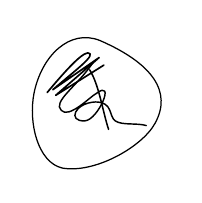
\begin{tikzpicture}[x=.012cm,y=-.012cm,line cap=round,line join=round]
\draw[line width=.45pt] (105,61) .. controls (73,48) and (43,77) .. (35,117)
 .. controls (29,148) and (39,190) .. (65,196)
 .. controls (99,202) and (149,174) .. (163,149)
 .. controls (182,115) and (160,85) .. (105,61);
\draw[line width=.52pt] (97,85) .. controls (81,109) and (54,126) .. (64,135)
 .. controls (72,144) and (95,120) .. (101,117)
 .. controls (122,101) and (103,145) .. (89,146)
 .. controls (70,147) and (78,127) .. (100,126)
 .. controls (119,126) and (114,141) .. (121,146)
 .. controls (128,151) and (144,148) .. (154,151);
\draw[line width=.55pt] (94,92) .. controls (104,108) and (108,137) .. (114,155);
\draw[line width=.60pt] (49,116) .. controls (65,97) and (84,75) .. (92,74)
 .. controls (103,75) and (78,93) .. (55,113)
 -- (104,79) -- (58,119) -- (109,87);
\end{tikzpicture}}}
de \(\Gamma\) sur \(\pi\) est \uline{très} non triviale (puisque
\(\chi:\Gamma\to\widehat{\mathbb Z}^{*}\) a une image ouverte !)
--- il \unsure{n'était} pas \(=\) évident a priori
\inserted{(sans raisons arithmétiques profondes !)} --- compte tenu de la structure
de \(\pi\) qu'on va donner --- qu'il existe de telles opérations de \(\Gamma\)
sur un \(\pi\) !

Cette condition \unsure{sera} complétée par une condition de non-trivialité à la Weil.

d) \(\exists\eta\in T^*\)\unsure{.} (une base de \(T\)), et des
\(\alpha_i\in\pi\) (afin de conjuguer \(\kappa_i\) en
\(\kappa'_i=\operatorname{int}(\alpha_i)\circ\kappa_i\))
\unsure{enfin} un entier \(g\geq0\) et des éléments
\(\unsure{x_i,y_i}\in\pi\) \((1\leq i\leq g)\), tels que l'on ait

\margin{84}

\scanpage{86}
\mspage{41}

1°) les \(\kappa'_i(\eta)\), \deleted{\illegible{1}} et les
\(\unsure{x_i,y_i|x_j,y_j}\) engendrent le groupe profini \(\pi\)

2°) Ils satisfont la relation
\[
\boxed{[x_1,y_1].[x_2,y_2]\ldots[x_g,y_g]\,
\kappa'_1(\eta)\kappa'_2(\eta)\ldots\kappa'_{\unsure{\nu|n}}(\eta)=1}
\]

3°) Cette relation, avec les générateurs envisagés décrit \(\pi\)
\inserted{(en tant que groupe profini)} par générateurs et relations\ldots

\uline{NB} On sait que par ces conditions, \(g\) est uniquement déterminé,
p.ex. par le fait que
\(\pi_{ab}/\deleted{\text{images des}}\sum\kappa_i(T)\)
est un \(\widehat{\mathbb Z}\)-module libre de rang \(2g\) --- \(\pi_{ab}\)
étant libre de rang \(2g+\nu-1\) où \(\nu=\operatorname{card}(I)\).

Pour le choix de \(\eta\), on sait que si \(\eta\) convient, alors
\(\forall\ \chi(\alpha)\eta\) aussi (où \(\alpha\in\Gamma\)) --- quitte à prendre
des conjugués. Donc les \(\eta\) qui conviennent \deleted{forment} contiennent
un sous-torseur\inserted{de \(T^*\)} (sous le ss-groupe ouvert
\(\chi(\Gamma)\) de \(\widehat{\mathbb Z}^{*}\).

\deleted{Supposons pour simplifier que \(g=0\) :
On voit donc que si le système des \(\kappa'_i(\eta)\) est un syst. de gén.
privilégié (au sens de d) ci-dessus) alors les
\(\operatorname{int}(g)\kappa'_i(\eta)\) aussi pour \(\forall g\in\mathcal E\),
[\unsure{\(=\)} \(\operatorname{int}(\alpha)\kappa'_i(\chi(g)\eta)\)
pour \(\alpha\in\pi\) convenable]}

\margin{85}

\scanpage{87}
\mspage{42}

\margin{(\unsure{donc|dans} \(\chi:\Gamma\to\widehat{\mathbb Z}^{*}\) \unsure{épi.})}

\deleted{donc aussi les \(\kappa'_i(\chi(g)\eta)\). \unsure{Prenant}
\(K=\mathbb Q\), on trouve donc par voie arithmétique :

\uline{Prop} Soit \(\pi\) le \unsure{\(P\)}-groupe libre
\inserted{de \unsure{\(\nu-1\)|\(\nu\) gén.}} \unsure{(}\uline{engendré} par des générateurs
\(\ell_1,\ldots,\ell_\nu\) satisfaisant la relation génératrice
\(\prod\ell_i=1\). Alors pour tout \(\alpha\in\widehat{\mathbb Z}^{*}\),
on a encore \(\prod\ell_i^\alpha=1\), et les \(\ell'_i=\ell_i^\alpha\)
avec cette relation décrivent le groupe profini \(\pi\).}
En fait, comme la structure du groupe \(\pi\) est indépendante de \(K\),
prenant \(K=\mathbb Q\) (et admettant qu'il existe une courbe lisse projective
géom. connexe de genre \(g\) sur \(\mathbb Q\), ayant \(\nu\) pts rat. / \(\mathbb Q\) !),
on trouve que si les \(\ell_i\), \deleted{\(\unsure{x_j,y_j}\)}
\((1\leq i\leq\nu\deleted{,\ \unsure{1\leq j\leq g}})\)
\deleted{conviennent, alors les} s'insèrent dans un syst. de générateurs
privilégié (avec des \(\unsure{x_\alpha,y_\alpha}\)) alors pour
\(\forall\rho\in\widehat{\mathbb Z}^{*}\), on peut trouver des conjugués
\(\ell'_i\) des \(\ell_i^\rho\) qui s'insèrent de \(=\).
Même pour \(\rho=-1\) ce n'est pas entièrement trivial\ldots

\deleted{\illegible{2}} Enfin, \unsure{on va} énoncer une condition
draconienne de non trivialité de l'opération de \(\Gamma\) sur \(\pi\).
Soit \(\mathcal E'\) un sous-groupe \inserted{\uline{ouvert} (donc}
d'indice fini) de \(\mathcal E\),
\inserted{\(\pi'=\pi\cap\mathcal E'=\operatorname{Ker}(\mathcal E'\to\Gamma')\)}
\deleted{\illegible{1} son image dans \unsure{\(\mathcal E\)|\(\Gamma\)}
(qui est ouvert dans \(\Sigma\)) de sorte que}

\margin{86}

\scanpage{88}

\(\Gamma'\) l'image de \(\mathcal E'\) dans \(\Gamma\). On trouve donc une
extension de \(\Gamma'\) \((=\operatorname{Gal}(\overline K'/K'))\) sur \(\pi'\),
donc aussi par \(\unsure{(\pi'_{ab})_{(\ell)}}\)
(\(\ell\) étant un nb premier), qui est (on le sait par d)) un
\(\mathbb Z_\ell\)-module libre de t.f.,
\inserted{sur lequel \(\Gamma'\) opère}

[Avec un peu de travail, on doit pouvoir mettre sur
\(\mathcal E'\to\Gamma\) une "structure à lacets" i.e. des
\(\mathcal E'_{i'}\), comme pour \(\mathcal E\), et décrire dans
\(\unsure{(\pi'_{ab})_{(\ell)}}\)
\inserted{la somme} des images des \deleted{\illegible{1}} \(L'_{i'}\),
sur lesquels \(\Gamma'\) opère \inserted{donc} via le caractère \(\chi\).

\margin{Ça se fait très élégamment dans le contexte
\diagram{\begin{tikzcd}[ampersand replacement=\&]
\Pi_{D^*} \arrow[r] \& \Pi_U \arrow[r] \& \Pi_e
\end{tikzcd}}}

On s'intéresse au quotient de \(\unsure{(\pi'_{ab})_{(\ell)}}\) par
\unsure{ce sous-module|ces sous-modules} relativement trivial (la partie "VA" du
module \(\ell\)-adique envisagé). Ceci posé

\textcircled{e} on exige que la représentation de \(\Gamma'\) là dessus soit
"pure de poids 1" --- \deleted{\unsure{i.e.} on ait} et que les polynômes car.
des frobénius (qui sont à coefficients \(\in\mathbb Z\), pas seulement
\(\in\mathbb Z_\ell\)) soient \uuline{indépendants} de \(\ell\).

\margin{\figure{\begin{tikzpicture}[x=1cm,y=1cm,line cap=round]
\draw[line width=.34pt] (.04,.30) .. controls (-.30,.35) and (-.42,.13) .. (-.40,-.08)
 .. controls (-.39,-.36) and (-.14,-.39) .. (.08,-.23)
 .. controls (.36,-.01) and (.28,.27) .. (.04,.30);
\node[inner sep=0pt] at (-.08,-.02) {$e$};
\draw[line width=.29pt] (-.06,-.71) .. controls (.01,-1.68) and (-.08,-2.52) .. (.02,-3.52)
 .. controls (.09,-4.37) and (.08,-5.24) .. (.15,-5.98)
 -- (.07,-6.30);
\end{tikzpicture}}}
\margin{87}

\scanpage{89}
\mspage{43}

\Needspace{4\baselineskip}
12. \uline{L'analogie topologique}\par\nobreak
Soit \(X\) une \deleted{variété}\inserted{surface} (topologique) compacte
orientable, \(S\) une partie finie de \(X\). Si \(X\) est connexe, on considère
l'ensemble \inserted{\unsure{\(\omega\)}} \unsure{des|ses} deux orientations,
on l'utilise pour tordre le groupe \(\mathbb Z\), d'où un groupe \unsure{\(T\)}
\[
T=\mathbb Z\mathop{\wedge}\limits_{\pm1}\unsure{\{\omega\}|\omega}.
\]
isomorphe (non canoniquement) à \(\mathbb Z\). Plus généralement, supposons
donné un tel groupe \(T\),
\inserted{i.e. un \(\omega\in\unsure{\operatorname{Ob}}\mathrm{Ens}_2\)}
--- une \(T\)-orientation de \(X\) sera par définition un \unsure{élém.}
de l'ens. \(\operatorname{Or}(X)\mathop{\wedge}\limits_{\{\pm1\}}\omega\).

[dans le cas précédent, \(X\) sera donc canoniquement \(T\)-orienté\ldots]

Considérons le groupoïde fondamental de \(X\setminus S=U\), soit \(\Pi_U\),
et le groupoïde fondamental \inserted{\(\Pi_{D^*}\)} des germes
d'espaces de \(X\) autour de \(S\), \uline{privé} de \(S\)
\inserted{\deleted{\unsure{des}} groupoïdes \unsure{?}}
(des germes de rev. universels de \(X\setminus S\) au voisinage de \(S\)).
On a donc un foncteur canonique
\diagram{\begin{tikzcd}[ampersand replacement=\&]
\unsure{\Pi_{D^*}} \arrow[r,dash] \& \Pi_U
\end{tikzcd}}
et d'autre part, \deleted{\illegible{2}} si \(X\) est \(T\)-orienté, on a une
structure supplémentaire

\margin{88}

\scanpage{90}

intéressante sur \inserted{le groupoïde} \(\Pi_{D^*}\) : le système local de
ses \(\pi_1\) est can. isom. à \(T\).

Associant à tout \(X\) \(T\)-orienté le système
\[
\Pi_{D^*}\longrightarrow\Pi_{\unsure{X|U}},\qquad
\kappa:T_{(\Pi_{D^*})}\simeq\pi_1(\Pi_{D^*}/e),
\]
on trouve une 2-équivalence entre la 2 catégorie topologique des
\deleted{\unsure{variétés}} couples \((X,S)\) d'une
\inserted{(pour les homéo. à isotopie près\ldots)}
\unsure{variété compacte \(T\)-orientée}, et de la 2-catégorie des systèmes
précédents \inserted{(pour les équivalences)}, \unsure{(}qui satisfont les conditions

a) \(\pi_0(\Pi_{D^*})\), \deleted{\unsure{et}} \(\pi_0(\Pi_X)\) finis

b) Pour \unsure{tte|\(\forall\)} composante connexe de \(\Pi_U\), soit
\(\Pi_{U_0}\), et la partie \(\unsure{\Pi_{D_0^*}}\) au dessus, explicitant la
situation \unsure{groupoïdes} par \unsure{un|une}
\inserted{groupe \(\pi\) et une} famille d'homs
\(T\xrightarrow{\kappa_i}\pi\), on a (\uline{NB} le tout \unsure{dépend|dépendant} de choix,
mais \(\pi\) est intrinsèque comme groupe extérieur, et les \(\kappa_i\)
\unsure{comme homs} extérieurs --- \unsure{définissent|définissant} une "\(T\)-structure à lacets
sur \(\unsure{S}\) ---) on a ce qui suit.

\margin{89}
